\section{MongoDB}

\subsection{Criação da base de dados}

\subsubsection{Motivação}

Por esta ser uma base de dados orientada a documentos, tem várias vantagens face ao MySQL, para além de ser escalável horizontalmente, é mais facil de manter, atualizar e é ótima para coletar informações referentes a um objeto, evitando joins de tabelas usados pelo MySQL visto este ter toda a informação de um objeto num mesmo documento.

\subsubsection{Criação - modificações}

Para a criação desta base de dados supusemos ser uma aplicação da loja na qual só se pretende obter informações sobre que utilizador consome filmes em que loja, quem o atendeu, em que data e qual o preço. Para além disso é importante saber as carateristicas dos filmes presentes nas lojas, as linguas em que estão, quais os atores que participaram e as categorias em que se insere,isto é, um sistema de suporte de consulta online.

\subsection{Criação - Estrutura da Base de Dados}

\par Em seguida apresentam-se os documentos gerados com base nos requisitos para a base de dados MongoDB.A coleção dos Filmes(films) contem o identificador do Filme(id), o titulo(title), o ano que saiu(release\_year), uma descrição do conteúdo do Filme(descrição), o Idioma original(original\_language), o Idioma estrangeiro(foreign\_language),um Array com as categorias as qual pertence(categorys) e , por último, uma lista de atores que participaram no filme(actors)\newline

\begin{lstlisting}[caption=Esquema da coleção films]
Filme:
{
	"id": , 
	"title": , 
	"release_year": , 
	"descricao": , 
	"original_language": , 
	"foreign_language": ,  
	"categorys": ,
	"actors":
}
\end{lstlisting}

A segunda coleção para os Pagamentos(payments) contem um objeto por loja que é identificado por um identificador(store\_id), contendo também o identificador do manager(manager\_id), um Array onde esta organizado as faturas por customer(paymentsByCostumer), cada elemento desse Array tem um identificador do cliente(customer\_id), o nome do mesmo (name), o email (email) e um Array de todas as faturas desse Cliente.

Cada fatura é identificado pelo seu identificador próprio(payment\_id), a quantia paga(amount), a data em qual foi efetuado(date), o identificador do staff que atendeu esse pagamento(staff\_id), o nome do staff(name) e o email do mesmo(email).

\begin{lstlisting}[caption=Esquema da coleção payments]
{
	"store_id" : ,
	"manager_id" : ,
	"paymentsByCostumer" : 
	[
		{
			"customer_id" : ,
			"name" : ,
			"email" : ,
			"payments" : 
			[
				{
					"staff_id" : ,
					"name" : ,
					"email" : ,
					"payment_id" : ,
					"amount" : ,
					"date" : 
				}
			]
		}
	]
}
\end{lstlisting}

\subsection{Preenchimento da Base de Dados}

A query usada para retirar os dados necessários para povoar o primeiro esquema mencionado na seção anterior é a seguinte.

\begin{lstlisting}[language=sql,caption=Query para povoar a primeira coleção]
SELECT f.title,f.release_year,f.description,c.name AS Category,
a.first_name,a.last_name, language.name AS Foreign_language,extra.name 
AS Original_language,
f.film_id 
 FROM film AS f LEFT JOIN film_category AS fc ON fc.film_id = f.film_id 
  LEFT JOIN category AS c ON c.category_id = fc.category_id 
   LEFT JOIN film_actor AS fa ON fa.film_id = f.film_id 
    LEFT JOIN actor AS a ON a.actor_id = fa.actor_id 
     LEFT JOIN language ON language.language_id = f.language_id 
      LEFT JOIN ( SELECT f.film_id,l.name FROM film AS f 
       LEFT JOIN language AS l ON l.language_id = f.original_language_id 
        WHERE f.original_language_id is not null) extra ON f.film_id = 
         extra.film_id
\end{lstlisting}

\par Em seguida podemos observar o loop usado para criar os documentos film.\newline
\begin{figure}[H]

  \centering

  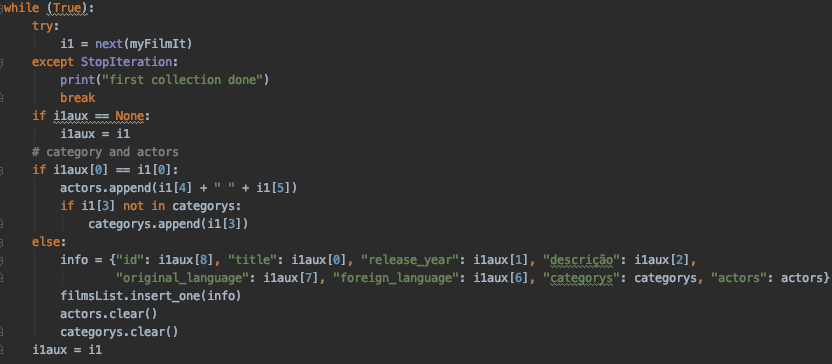
\includegraphics[scale = 0.45]{ciclo.png}

  \caption {Ciclo que gera cada documento Film guardado na base de dados MongoDB}

  \label {fig1}

\end{figure}

Cada objeto iterado neste ciclo while corresponde a um film, podendo haver filmes repetidos em iterações sucessivas cuja única diferença reside sempre no ator e pode ter também diferentes categorias, tendo portanto, cada iteração, um ator diferente e uma ou nenhuma categoria. Assim fazendo uso do ciclo com a verificação do id de cada filme sendo igual permite que identifiquemos o mesmo filme em várias iterações e possamos adicionar os atores todos numa string bem como as categorias. Quando a verificação da igualdade do filme falha sabemos que podemos adicionar o filme á base de dados pois já coletámos todos os atores e categorias deste.

A segunda query usada para povoar a coleção payments foi a seguinte:

\begin{lstlisting}[language=sql,caption=Query para povoar a segunda coleção]
SELECT s.store_id, c.first_name AS Costumer_first_name,
c.last_name AS Costumer_last_name, p.amount, p.payment_date, 
st.first_name AS Staff_first_name, st.last_name  
AS Staff_last_name,s.manager_staff_id,st.staff_id,st.email,
p.payment_id,c.customer_id,c.email FROM 
 store AS s LEFT JOIN customer AS c ON s.store_id = s.store_id 
  LEFT JOIN payment AS p ON c.customer_id = p.customer_id 
   LEFT JOIN staff AS st ON p.staff_id = st.staff_id
\end{lstlisting}

O ciclo parecido ao anterior coleta as informações de cada linha devolvida pela query anterior. Seguidamente, verifica caso existe já um objeto corresponde ao store\_id devolvido.Caso não exista, cria esse documento. Posteriormente faz o mesmo com os clientes e com os pagamentos por essa ordem. Atualizando os arrays correspondentes de cada.

\begin{figure}[H]

  \centering

  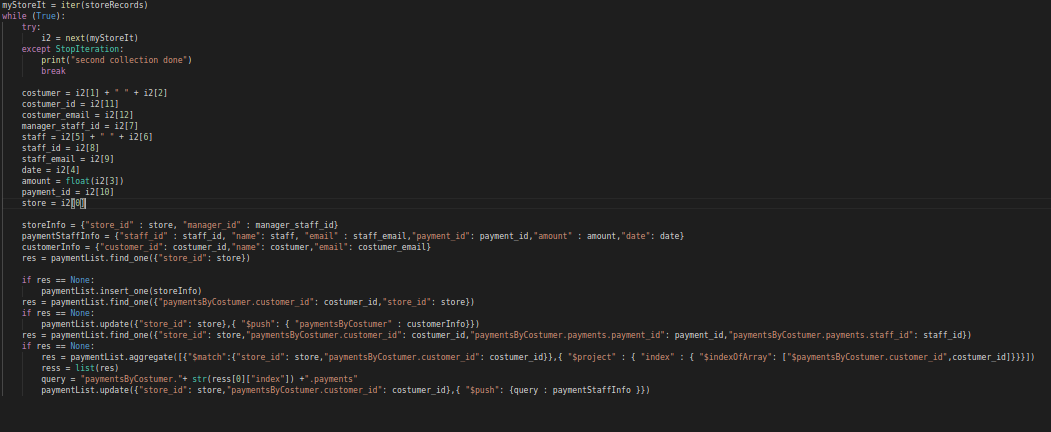
\includegraphics[width=\textwidth]{PovoamentoMongo2.png}

  \caption {Ciclo que gera cada documento Store guardado na base de dados MongoDB}

  \label {fig:Mongo2}

\end{figure}



\subsection{Querys a Base de Dados}

Em seguida listam-se algumas das querys feitas á base de dados Mongo e as respetivas respostas.Primeiramente, uma query simples que devolve todos os titulos e as linguagens que tem todos os filmes.Poder-se-ia , facilmente, filtrar por qualquer dos campos presentes na coleção films.

\begin{lstlisting}[language=java,caption=Query ao Mongo para devolver todos os Filmes]
filmsList.find({},
{
	"title": 1, 
	"original\_language": 1, 
	"foreign\_language": 1, "\_id": 0
})
\end{lstlisting}

Por exemplo, a seguinte query devolve todos os titúlos dos filmes que tenha sido estreados depois do ano 2005.E, também, uma query para determinar os titúlos dos filmes da categoria Action.

\begin{lstlisting}[language=java,caption=Query ao Mongo para devolver todos os Filmes estreados depois de 2005]

db.films.find(
{
	"release_year": {$gt : 2005}
},
{
	"title":1
})

\end{lstlisting}

\begin{lstlisting}[language=java,caption=Query ao Mongo para devolver todos os Filmes da Categoria Action]

db.films.find(
{
	"categorys": "Action"
},
{
	"title":1
})
\end{lstlisting}

Finalmente, uma query realizada a coleção payments.Esta query usa o aggregate para fazer "unwind" de um dos arrays presentes na coleção payments.De seguida, filtra só por aqueles que tem o customer\_id igual ao desejado.E,concluindo, devolve objetos que contem os identificadores da store e todos pagamentos realizados pelo Cliente.

\begin{lstlisting}[language=java,caption=Query para obter as faturas de um dado Cliente organizado por Store]

db.payments.aggregate(
[{"$unwind": "$paymentsByCostumer"},
 {"$match":{"paymentsByCostumer.customer_id" : 1}},
 {"$project" :{"store_id":"$store_id",
 "payments":"$paymentsByCostumer.payments"}}])

\end{lstlisting}

Note-se que este tipo de queries já é mais trabalhosa para o Mongo.
